\begin{itemize}
    \item La clasificación es fundamental tanto para la inteligencia humana como para la artificial.
    \item Decidir qué letra, palabra o imagen se ha presentado a nuestros sentidos, reconocer caras o voces, clasificar el correo, asignar calificaciones a las tareas.
    \item Estos son ejemplos de asignar una categoría a una entrada.
    \item El objetivo de la clasificación es tomar una única observación, extraer algunas características útiles y así clasificar la observación en una de las clases discretas establecidas.
    \item La mayoría de los casos de clasificación en el procesamiento del lenguaje se realizan mediante aprendizaje automático supervisado.
    \item Estas diapositivas se basan en el material del curso de Daniel Jurafsky: \url{https://web.stanford.edu/~jurafsky/slp3/4.pdf}
\end{itemize}

Ejemplo 1: Clasificación de spam

\begin{figure}[h]

\includegraphics[scale = 0.35]{pics/spam.png}
\end{figure}


Ejemplo 2: ¿Quién escribió los documentos Federalist?

\begin{itemize}
    \item 1787-8: Ensayos anónimos intentaron convencer a Nueva York de ratificar la Constitución de EE. UU.: Jay, Madison, Hamilton.
    \item La autoría de 12 de las cartas está en disputa.
    \item 1963: Resuelto por Mosteller y Wallace mediante métodos bayesianos.
\end{itemize}

\begin{center}
    \begin{figure}[h]
        \begin{minipage}{0.3\textwidth}
            \centering
            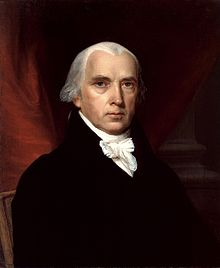
\includegraphics[width=\linewidth]{pics/madison.png}
            \caption{James Madison}
        \end{minipage}\hfill
        \begin{minipage}{0.3\textwidth}
            \centering
            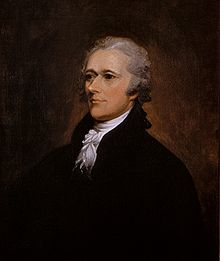
\includegraphics[width=\linewidth]{pics/hamilton.png}
            \caption{Alexander Hamilton}
        \end{minipage}
    \end{figure}
\end{center}


Ejemplo 3: ¿Cuál es el tema de este artículo médico?

\begin{figure}[h]
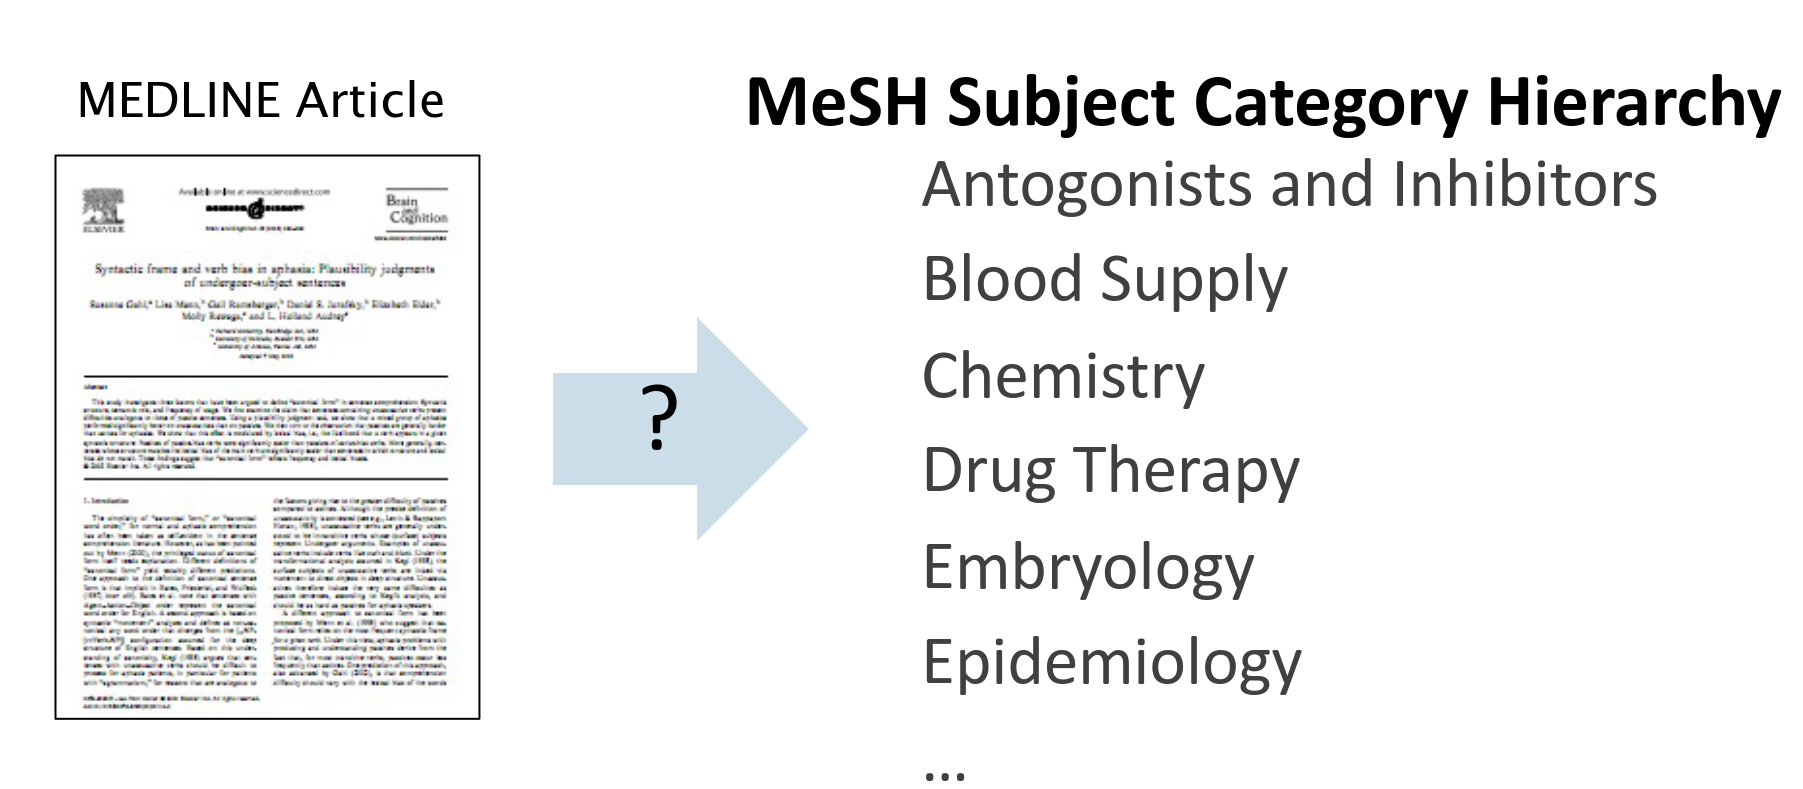
\includegraphics[scale = 0.2]{pics/medarticle.png}
\end{figure}



Ejemplo 4: ¿Reseña de película positiva o negativa?

\begin{itemize}
    \item \textcolor{blue}{\textbf{+}} ...personajes extravagantes y sátira \textcolor{blue}{rico} aplicada, y algunos \textcolor{blue}{grandes} giros de la trama.
    \item \textcolor{red}{\textbf{-}} Fue \textcolor{red}{patético}. La peor parte fue las escenas de boxeo...
    \item \textcolor{blue}{\textbf{+}} ...salsa de caramelo \textcolor{blue}{increíble} y almendras dulces y tostadas. ¡Me \textcolor{blue}{encanta} este lugar!
    \item \textcolor{red}{\textbf{-}} ...pizza \textcolor{red}{horrible} y \textcolor{red}{ridículamente} cara...
\end{itemize}



\paragraph{¿Por qué el análisis de sentimientos?}

\begin{itemize}
    \item Película: ¿Esta reseña es positiva o negativa?
    \item Productos: ¿Qué opinan las personas sobre el nuevo iPhone?
    \item Sentimiento público: ¿Cómo está la confianza del consumidor?
    \item Política: ¿Qué opinan las personas sobre este candidato o tema?
    \item Predicción: Predecir resultados electorales o tendencias del mercado a partir del sentimiento.
\end{itemize}


\paragraph{Clasificación básica de sentimientos}

El análisis de sentimientos es la detección de actitudes.

\begin{itemize}
    \item Tarea simple en la que nos enfocamos en esta clase.
    \begin{itemize}
        \item ¿Es la actitud de este texto positiva o negativa?
    \end{itemize}
\end{itemize}



\paragraph{Resumen: Clasificación de texto}

La clasificación de texto se puede aplicar a varias tareas, incluyendo:

\begin{itemize}
    \item Análisis de sentimientos
    \item Detección de spam
    \item Identificación de autoría
    \item Identificación de idioma
    \item Asignación de categorías, temas o géneros
    \item ...
\end{itemize}


\section{Clasificación de texto: Definición}

\textbf{Entrada}:
\begin{itemize}
    \item Un documento $d$
    \item Un conjunto fijo de clases $C = \{c_1, c_2, \ldots, c_J\}$
\end{itemize}

\textbf{Salida}: Una clase predicha $c \in C$


\subsection{Métodos de clasificación: Reglas codificadas a mano}

Reglas basadas en combinaciones de palabras u otras características.

\begin{itemize}
    \item Spam: \textit{dirección-en-lista-negra} O (\textit{“dólares” Y “has sido seleccionado”})
    \item La precisión puede ser alta si las reglas se refinan cuidadosamente por expertos
    \item Pero construir y mantener estas reglas es costoso
\end{itemize}

\subsection{Métodos de clasificación: Aprendizaje automático supervisado}

\textbf{Entrada}:
\begin{itemize}
    \item Un documento $d$
    \item Un conjunto fijo de clases $C = \{c_1, c_2, \ldots, c_J\}$
    \item Un conjunto de entrenamiento de $m$ documentos etiquetados manualmente: $(d_1, c_1), (d_2, c_2), \ldots, (d_m, c_m)$
\end{itemize}

\textbf{Salida}:
\begin{itemize}
    \item Un clasificador aprendido $\gamma: d \to c$
\end{itemize}

Cualquier tipo de clasificador se puede utilizar:
\begin{itemize}
    \item Naïve Bayes
    \item Regresión logística
    \item Redes neuronales
    \item k-vecinos más cercanos
    % Agrega más clasificadores según sea necesario
\end{itemize}

\subsection{Problemas de aprendizaje supervisado}
\begin{itemize}
    \item Tenemos ejemplos de entrenamiento $x^{(i)}$, $y^{(i)}$ para $i = 1, \ldots, m$. Cada $x^{(i)}$ es una entrada, cada $y^{(i)}$ es una etiqueta.
    \item La tarea es aprender una función $f$ que asigna las entradas $x$ a las etiquetas $f(x)$.
    \item Modelos condicionales:
    \begin{itemize}
        \item Aprender una distribución $p(y|x)$ a partir de ejemplos de entrenamiento.
        \item Para cualquier entrada de prueba $x$, definir $f(x) = \arg \max_y p(y|x)$.
    \end{itemize}
\end{itemize}

\subsection{Modelos generativos}
\begin{itemize}
    \item Dados ejemplos de entrenamiento $x^{(i)}$, $y^{(i)}$ para $i = 1, \ldots, m$, la tarea es aprender una función $f$ que asigna las entradas $x$ a las etiquetas $f(x)$.
    \item Modelos generativos:
    \begin{itemize}
        \item Aprender la distribución conjunta $p(x, y)$ a partir de los ejemplos de entrenamiento.
        \item A menudo, tenemos $p(x, y) = p(y)p(x|y)$.
        \item Nota: Luego tenemos
        \[
        p(y|x) = \frac{p(y)p(x|y)}{p(x)} \quad \text{donde} \quad p(x) = \sum_y p(y)p(x|y).
        \]
    \end{itemize}
\end{itemize}

\subsection{Clasificación con Modelos Generativos}
\begin{itemize}
    \item Dados ejemplos de entrenamiento $x^{(i)}$, $y^{(i)}$ para $i = 1, \ldots, m$. La tarea consiste en aprender una función $f$ que mapee las entradas $x$ a las etiquetas $f(x)$.
    \item Modelos generativos:
    \begin{itemize}
        \item Aprenden la distribución conjunta $p(x, y)$ a partir de los ejemplos de entrenamiento.
        \item A menudo, tenemos $p(x, y) = p(y)p(x|y)$.
    \end{itemize}
    \item La salida del modelo es:
    \[
    \begin{aligned}
    f(x) = \arg\max_y p(y|x) &= \arg\max_y \frac{p(y)p(x|y)}{p(x)} \\
    &= \arg\max_y p(y)p(x|y)
    \end{aligned}
    \]
\end{itemize}


\section{Intuición del Bayes Ingenuo}
El Bayes Ingenuo es un método de clasificación simple ("ingenuo") basado en la regla de Bayes.
\begin{itemize}
    \item Se basa en una representación muy simple de un documento: \textit{Bolsa de palabras}.
\end{itemize}

\paragraph{La Representación de Bolsa de Palabras}

\begin{figure}[h]
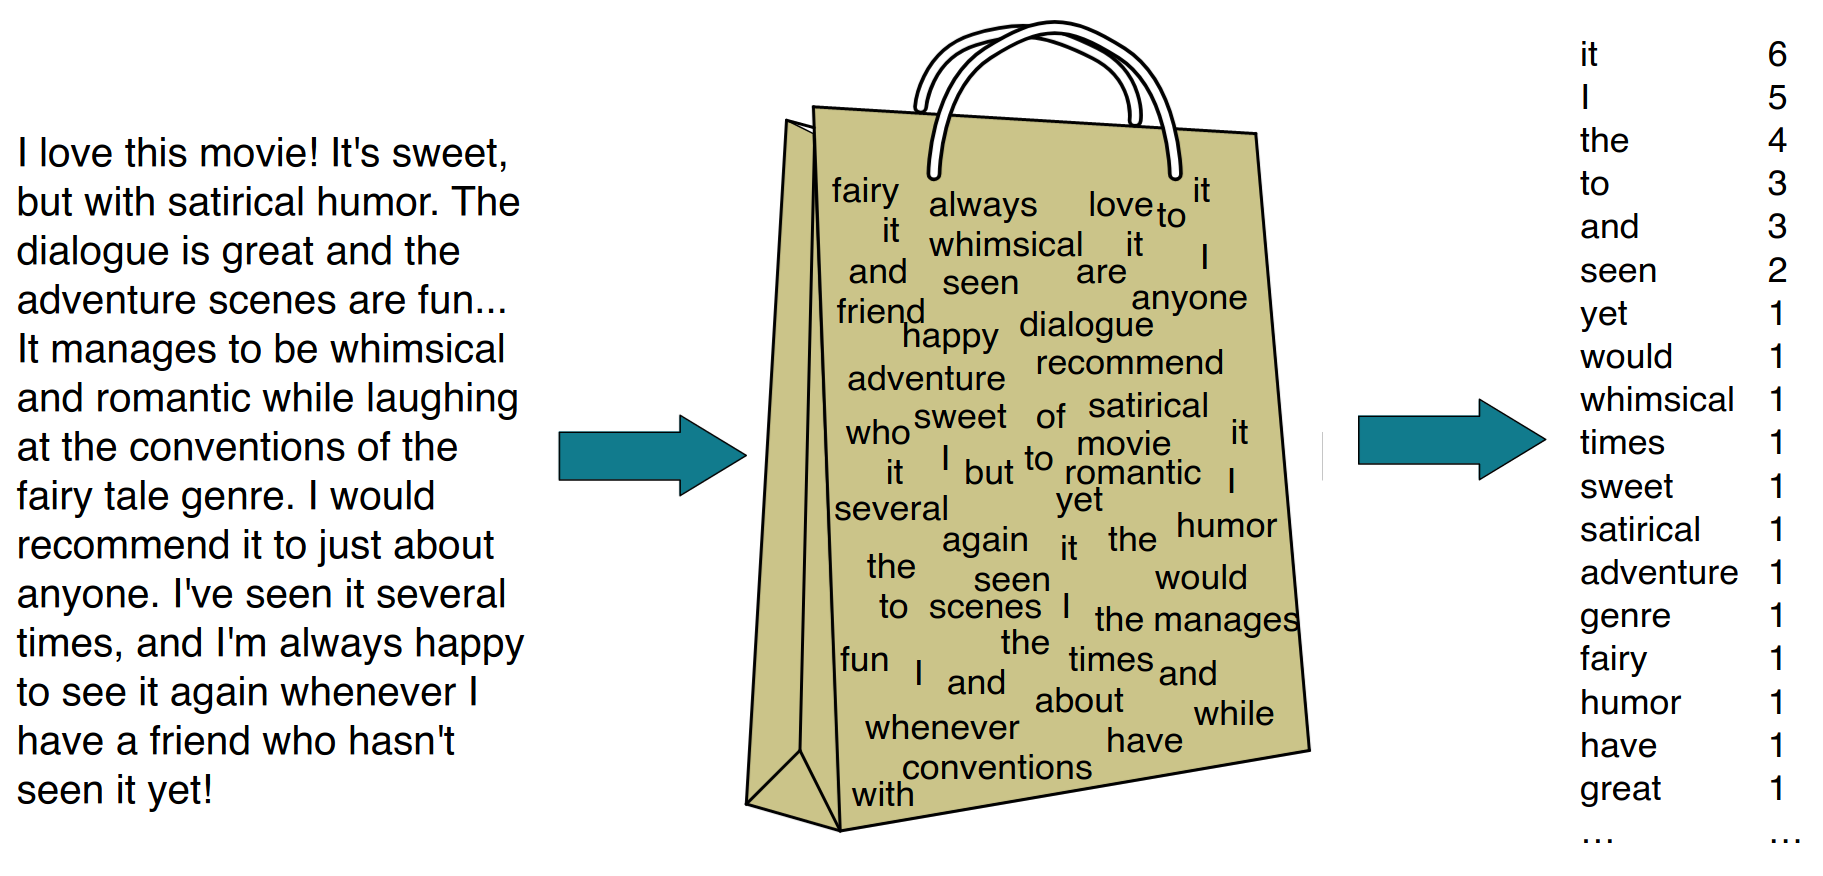
\includegraphics[scale = 0.22]{pics/bow.png}
\end{figure}


\subsection{Aplicación de la Regla de Bayes a Documentos y Clases}
Para un documento $d$ y una clase $c$:
\[
P(c | d) = \frac{P(d | c)P(c)}{P(d)}
\]


\section{Clasificador Bayes Ingenuo}
\begin{itemize}
    \item MAP significa "máximo a posteriori," que representa la clase más probable:
    \[
    c_{\text{MAP}} = \arg\max_{c \in C} P(c | d)
    \]
    \item Para calcular la clase más probable, aplicamos la regla de Bayes:
    \[
    = \arg\max_{c \in C} \frac{P(d | c)P(c)}{P(d)}
    \]
    \item Finalmente, podemos eliminar el denominador ya que permanece constante para todas las clases:
    \[
    = \arg\max_{c \in C} P(d | c)P(c)
    \]
    \item Para clasificar el documento $d$, usamos la estimación MAP:
    \[
    c_{\text{MAP}} = \arg\max_{c \in C} P(d | c)P(c)
    \]
    \item El documento $d$ se representa como un conjunto de características $x_1, x_2, \ldots, x_n$.
    \item El clasificador calcula la probabilidad condicional de las características dada una clase y la probabilidad a priori de la clase:
    \[
    = \arg\max_{c \in C} P(x_1, x_2, \ldots, x_n | c)P(c)
    \]
    \item El término $P(x_1, x_2, \ldots, x_n | c)$ representa la

 "verosimilitud" de las características dada la clase.
    \item El término $P(c)$ representa la probabilidad "a priori" de la clase.
    \item El clasificador Bayes Ingenuo \cite{mccallum1998comparison} calcula la estimación MAP considerando las probabilidades de verosimilitud y a priori:
    \[
    c_{\text{MAP}} = \arg\max_{c \in C} P(x_1, x_2, \ldots, x_n | c)P(c)
    \]
    \item La probabilidad de las características dada la clase, $P(x_1, x_2, \ldots, x_n | c)$, puede estimarse contando las frecuencias relativas en un corpus.
    \item La probabilidad a priori de la clase, $P(c)$, representa con qué frecuencia ocurre esta clase.
    \item Sin algunas suposiciones simplificadoras, estimar la probabilidad de cada posible combinación de características en $P(x_1, x_2, \ldots, x_n | c)$ requeriría un gran número de parámetros y conjuntos de entrenamiento imposiblemente grandes.
    \item Por lo tanto, los clasificadores Bayes Ingenuo realizan dos suposiciones simplificadoras.
\end{itemize}


\subsection{Suposiciones de Independencia del Bayes Ingenuo Multinomial}
\begin{itemize}
    \item Suposición de Bolsa de Palabras: asumimos que la posición de las palabras en el documento no importa.
    \item Suposición de Independencia Condicional: asumimos que las probabilidades de las características $P(x_i | c_j)$ son independientes dada la clase $c_j$.
    \item En el clasificador Bayes Ingenuo Multinomial, la probabilidad de un documento con características $x_1, x_2, \ldots, x_n$ dada la clase $c$ se puede calcular como:
    \[
    P(x_1, x_2, \ldots, x_n | c) = P(x_1 | c) \cdot P(x_2 | c) \cdot P(x_3 | c) \cdot \ldots \cdot P(x_n | c)
    \]
\end{itemize}

\subsection{Clasificador Bayes Ingenuo Multinomial}
\begin{itemize}
    \item La estimación del Máximo A Posteriori (MAP) para la clase $c$ en el clasificador Bayes Ingenuo Multinomial se calcula como:
    \[
    c_{\text{MAP}} = \arg\max_{c \in C} P(x_1, x_2, \ldots, x_n | c)P(c)
    \]
    \item Alternativamente, podemos escribirlo como:
    \[
    c_{\text{NB}} = \arg\max_{c \in C} P(c_j) \prod_{x \in X} P(x | c)
    \]
    \item $P(c_j)$ representa la probabilidad a priori de la clase $c_j$.
    \item $\prod_{x \in X} P(x | c)$ representa la verosimilitud de las características $x_1, x_2, \ldots, x_n$ dadas la clase $c$.
\end{itemize}


\subsection{Aplicación de los clasificadores Naive Bayes multinomiales a la clasificación de texto}

El clasificador Naive Bayes multinomial para la clasificación de texto se puede aplicar de la siguiente manera:
\[
c_{\text{NB}} = \arg\max_{c_j \in C} P(c_j) \prod_{i \in \text{positions}} P(x_i | c_j)
\]
Donde:
\begin{itemize}
    \item $c_{\text{NB}}$ representa la clase predicha para el documento de prueba.
    \item $C$ es el conjunto de todas las clases posibles.
    \item $P(c_j)$ es la probabilidad previa de la clase $c_j$.
    \item $\prod_{i \in \text{positions}} P(x_i | c_j)$ calcula la probabilidad de cada característica $x_i$ en la posición $i$ dada la clase $c_j$.
    \item El producto se toma sobre todas las posiciones de palabras en el documento de prueba.
\end{itemize}

\subsection{Problemas al multiplicar muchas probabilidades}

Multiplicar muchas probabilidades puede resultar en un desbordamiento de punto flotante, especialmente cuando se manejan probabilidades pequeñas. Por ejemplo, $0.0006 \times 0.0007 \times 0.0009 \times 0.01 \times 0.5 \times 0.000008 \ldots$.

Para solucionar este problema, podemos utilizar logaritmos, ya que $\log(ab) = \log(a) + \log(b)$. En lugar de multiplicar las probabilidades, podemos sumar los logaritmos de las probabilidades. Así, el clasificador Naive Bayes multinomial se puede expresar utilizando logaritmos de la siguiente manera:
\[
c_{\text{NB}} = \arg\max_{c_j \in C} \left(\log(P(c_j)) + \sum_{i \in \text{position}} \log(P(x_i | c_j))\right)
\]

Al tomar logaritmos, evitamos el problema del desbordamiento de punto flotante y realizamos cálculos en el espacio logarítmico. El clasificador se convierte en un modelo lineal, donde la predicción es el argmax de la suma de pesos (logaritmos de probabilidades) y las entradas (logaritmos de probabilidades condicionales). Por lo tanto, Naive Bayes es un clasificador lineal que opera en el espacio logarítmico.

\subsection{Aprendizaje del modelo Naive Bayes multinomial}

El primer intento: Estimaciones de máxima verosimilitud
\begin{itemize}
    \item Las probabilidades se estiman utilizando las frecuencias observadas en los datos de entrenamiento.
    \item La probabilidad previa de una clase $c_j$ se estima como:
    \[
    \hat{P}(c_j) = \frac{N_{c_j}}{N_{\text{total}}}
    \]
    donde $N_{c_j}$ es el número de documentos en la clase $c_j$ y $N_{\text{total}}$ es el número total de documentos.
    \item La estimación de la probabilidad de la palabra $w_i$ dada la clase $c_j$ se calcula como:
    \[
    \hat{P}(w_i | c_j) = \frac{{\text{count}(w_i, c_j)}}{\sum_{w\in V}{\text{count}(w, c_j)}}
    \]
    donde $w \in V$ representa una palabra en el vocabulario $V$.
    \item El denominador es la suma de las frecuencias de todas las palabras en el vocabulario dentro de la clase $c_j$.
\end{itemize}

\subsection{Estimación de parámetros}

Para estimar los parámetros del modelo Naive Bayes multinomial, seguimos estos pasos:

\begin{itemize}
  \item Creamos un mega-documento para cada tema $c_j$ concatenando todos los documentos de ese tema.
  \item Calculamos la frecuencia de la palabra $w_i$ en el mega-documento, que representa la fracción de veces que la palabra $w_i$ aparece entre todas las palabras en los documentos del tema $c_j$.
  \item La probabilidad estimada $\hat{P}(w_i | c_j)$ de la palabra $w_i$ dada la clase $c_j$ se obtiene dividiendo el recuento de ocurrencias de $w_i$ en el mega-documento del tema $c_j$ por el recuento total de palabras en el mega-documento:
  \[
  \hat{P}(w_i | c_j) = \frac{{\text{count}(w_i, c_j)}}{\sum_{w\in V}{\text{count}(w, c_j)}}
  \]
  Aquí, $\text{count}(w_i, c_j)$ representa el número de veces que la palabra $w_i$ aparece en el mega-documento del tema $c_j$, y $\text{count}(w, c_j)$ es el recuento total de palabras en el mega-documento.
\end{itemize}

\subsection{Probabilidades cero y el problema de las palabras no vistas}

Consideremos el escenario en el que no hemos encontrado la palabra "fantástico" en ningún documento de entrenamiento clasificado como positivo (pulgar hacia arriba). Utilizando la estimación de máxima verosimilitud, la probabilidad $\hat{P}(\text{``fantástico''} \mid \text{positivo})$ se calcularía como:
\[
\hat{P}(\text{``fantástico''} \mid \text{positivo}) = \frac{\text{count}(\text{``fantástico''}, \text{positivo})}{\sum_{w \in V} \text{count}(w, \text{positivo})}
\]

En este caso, el recuento de la palabra ``fantástico'' en los documentos positivos es cero, lo que conduce a una probabilidad cero:
\[
\hat{P}(\text{``fantástico''} \mid \text{positivo}) = \frac{0}{\sum_{w \in V} \text{count}(w, \text{positivo})} = 0
\]

Sin embargo, las probabilidades cero no pueden eliminarse, independientemente de la evidencia adicional presente. Esto plantea un problema al calcular la estimación del máximo a posteriori (MAP), que se utiliza para la clasificación:
\[
c_{\text{MAP}} = \arg\max_c \left(\hat{P}(c) \prod_{i} \hat{P}(x_i \mid c)\right)
\]

Con una probabilidad cero para una palabra, toda la expresión se vuelve cero, independientemente de la otra evidencia.

\subsection{Suavizado Laplaciano (Add-1) para Naïve Bayes}

Manejo de probabilidades cero con el suavizado Laplaciano (Add-1):
\begin{itemize}
    \item Para abordar el problema de las probabilidades cero, podemos utilizar la técnica de suavizado Laplaciano (Add-1).
    \item La estimación suavizada $\hat{P}(w_i \mid c)$ se calcula como:
    \[
    \hat{P}(w_i \mid c) = \frac{\text{count}(w_i, c) + 1}{\sum_{w \in V} (\text{count}(w, c) + 1)}
    \]
    \item Aquí, se agrega un recuento adicional de 1 tanto al numerador como al denominador.
    \item El denominador se ajusta agregando el tamaño del vocabulario $V$ para garantizar una normalización adecuada.
    \item Al hacerlo, evitamos las probabilidades cero y permitimos que cierta masa de probabilidad se distribuya a palabras no vistas.
    \item Esta técnica de suavizado ayuda a mitigar el problema de las palabras no vistas y evita la eliminación completa de ciertas clases durante la clasificación.
\end{itemize}

\subsection{Naïve Bayes multinomial: aprendizaje}

Aprendiendo el modelo Naïve Bayes multinomial:
\begin{itemize}
    \item Para aprender los parámetros del modelo, necesitamos calcular los términos $P(c_j)$ y $P(w_k \mid c_j)$.
    \item Para cada clase $c_j$ en el conjunto de clases $C$, realizamos los siguientes pasos:
    \begin{itemize}
        \item Recuperamos todos los documentos $docs_j$ que pertenecen a la clase $c_j$.
        \item Calculamos el término $P(w_k \mid c_j)$ para cada palabra $w_k$ en el vocabulario $V$:
        \[
        P(w_k \mid c_j) = \frac{{n_k + \alpha}}{{n + \alpha \cdot \lvert \text{Vocabulary} \rvert}}
        \]
        donde $n_k$ representa el número de ocurrencias de la palabra $w_k$ en el documento concatenado $Text_j$.
        \item Calculamos la probabilidad a priori $P(c_j)$:
        \[
        P(c_j) = \frac{{\lvert docs_j \rvert}}{{\lvert \text{total number of documents} \rvert}}
        \]
    \end{itemize}
    \item Para calcular $P(w_k \mid c_j)$, necesitamos extraer el vocabulario $V$ del corpus de entrenamiento.
\end{itemize}

\subsection{Palabras desconocidas}

Tratamiento de palabras desconocidas en los datos de prueba:
\begin{itemize}
    \item Cuando encontramos palabras desconocidas en los datos de prueba que no aparecen en los datos de entrenamiento o en el vocabulario, las ignoramos.
    \item Eliminamos estas palabras desconocidas del documento de prueba como si no estuvieran presentes en absoluto.
    \item No asignamos ninguna probabilidad a estas palabras desconocidas en el proceso de clasificación.
\end{itemize}

Esto es una visión general del modelo Naive Bayes multinomial y su aplicación a la clasificación de texto. Cabe destacar que existen variantes y extensiones más sofisticadas de Naive Bayes que se adaptan a diferentes requisitos y características de los datos.


\section{Ejemplo}

\textbf{Datos de Entrenamiento:} 

\begin{table}[h]
\centering
\begin{tabular}{|c|p{0.7\textwidth}|}
\hline
\textbf{Categoría} & \textbf{Texto} \\
\hline
Negative & Just plain boring, entirely predictable and lacks energy. \\
\hline
Negative & No surprises and very few laughs. \\
\hline
Positive & Very powerful. \\
\hline
Positive & The most fun film of the summer. \\
\hline
\end{tabular}
\end{table}


\textbf{Test:} 
\begin{table}[h]
\centering
\begin{tabular}{|c|p{0.7\textwidth}|}
\hline
\textbf{Categoría} & \textbf{Texto} \\
\hline
? & Predictable with no fun. \\
\hline
\end{tabular}
\end{table}

\begin{figure}[h]
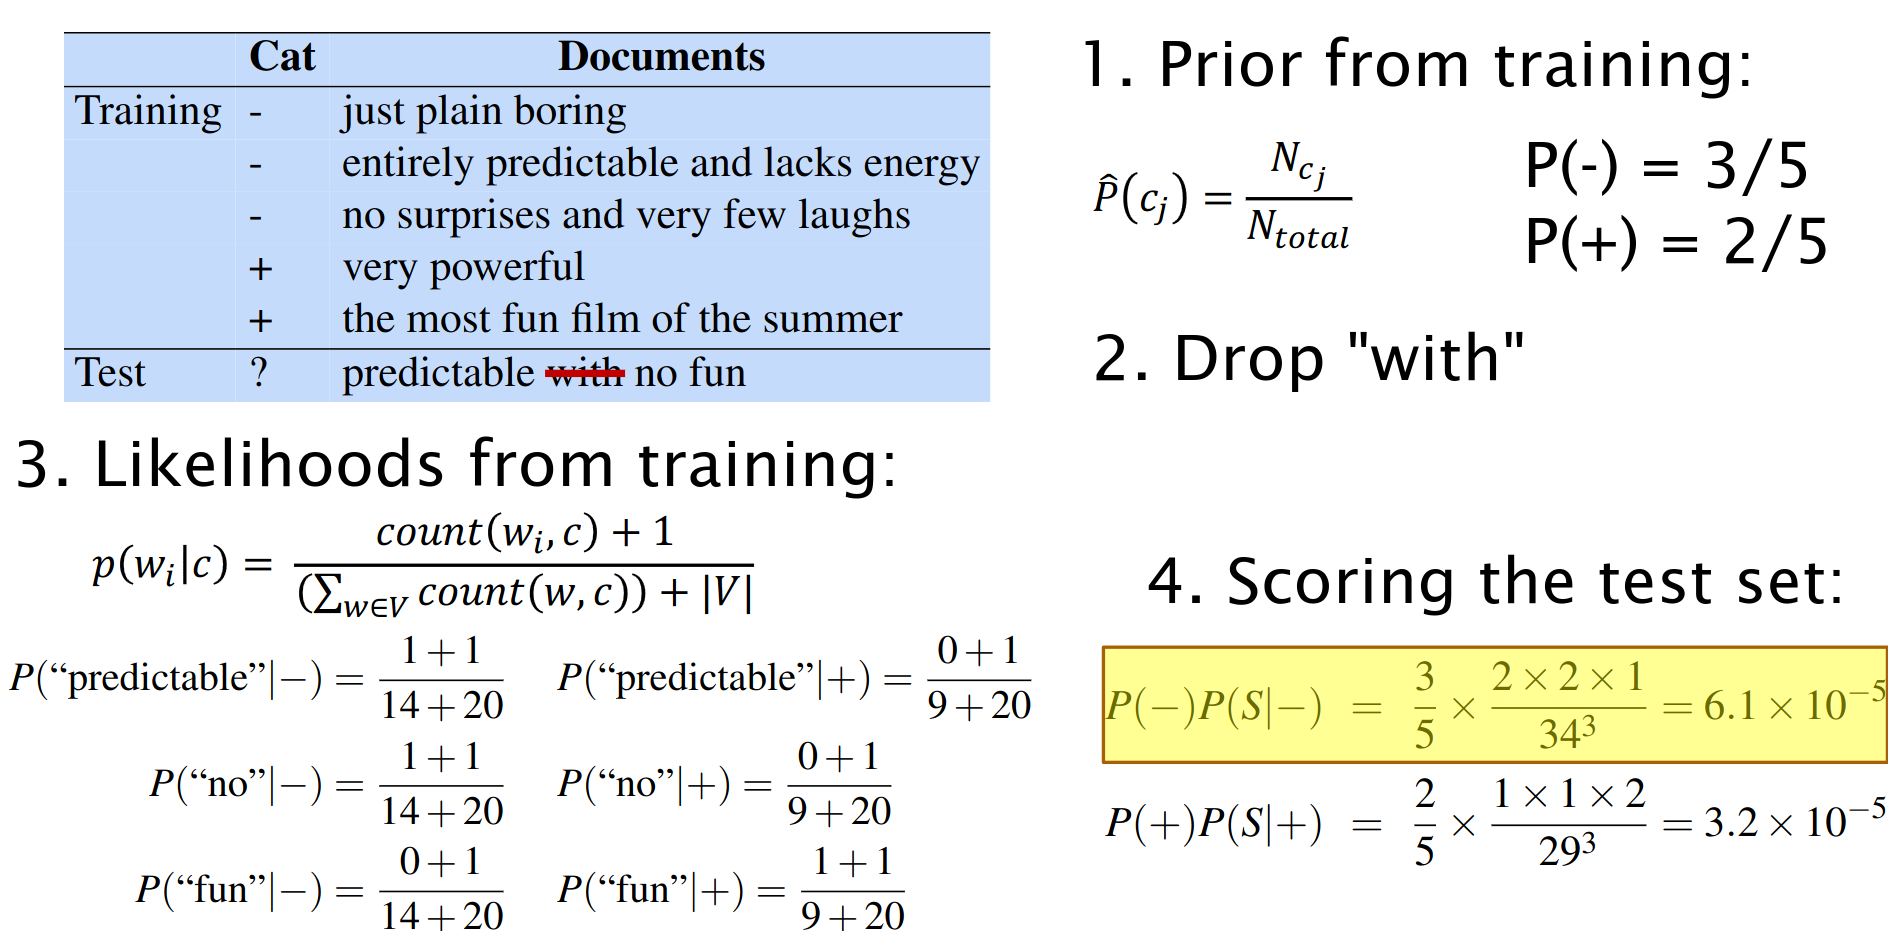
\includegraphics[scale = 0.23]{pics/naive_example.png}
\end{figure}


%Translate this Latex book chapter to Spanish. Output in latex format. Turn bullet points (items) into full paragraphs when appropriate:

\section{Naive Bayes como modelo de lenguaje}

Cuando utilizamos características de palabras individuales y consideramos todas las palabras en el texto, el naive Bayes tiene una similitud importante con la modelización del lenguaje.

Específicamente, un modelo naive Bayes se puede ver como un conjunto de modelos de lenguaje de unigramas específicos de cada clase, en el que el modelo para cada clase instancia un modelo de lenguaje de unigrama.

Las características de verosimilitud del modelo naive Bayes asignan una probabilidad a cada palabra $P(\text{word}|c)$, y el modelo también asigna una probabilidad a cada oración:

\[P(s|c) = \prod_{i\in \text{positions}} P(w_i|c)\]

Consideremos un modelo naive Bayes con las clases positiva (+) y negativa (-) y los siguientes parámetros del modelo:

\begin{center}
\begin{tabular}{ccc}
\textbf{w} & $P(w|+)$ & $P(w|-)$ \\
I & 0.1 & 0.2 \\
love & 0.1 & 0.001 \\
this & 0.01 & 0.01 \\
fun & 0.05 & 0.005 \\
film & 0.1 & 0.1 \\
... & ... & ...
\end{tabular}
\end{center}

Cada una de las dos columnas anteriores instancian un modelo de lenguaje que puede asignar una probabilidad a la oración "I love this fun film":

\[P("\text{I love this fun film}"|+) = 0.1 \times 0.1 \times 0.01 \times 0.05 \times 0.1 = 0.0000005\]
\[P("\text{I love this fun film}"|-) = 0.2 \times 0.001 \times 0.01 \times 0.005 \times 0.1 = 0.0000000010\]

Como sucede, el modelo positivo asigna una probabilidad más alta a la oración:
\[P(s|\text{pos}) > P(s|\text{neg})\]

Cabe destacar que esto es solo la parte de verosimilitud del modelo naive Bayes; una vez que multiplicamos por la probabilidad a priori, un modelo naive Bayes completo podría tomar una decisión de clasificación diferente.





\section{Evaluation}

\begin{itemize}
 \item Let's consider just binary text classification tasks. 
 \item Imagine you're the CEO of Delicious Pie Company. 
\item You want to know what people are saying about your pies. 
\item So you build a "Delicious Pie" tweet detector with the following classes:
\begin{itemize}
\item Positive class: tweets about Delicious Pie Co
\item Negative class: all other tweets
\end{itemize}
\end{itemize}



\subsection{The 2-by-2 Confusion Matrix}
\begin{table}[h]
\centering
\begin{tabular}{|c|c|c|}
\hline
\textbf{} & \textbf{System Positive} & \textbf{System Negative} \\
\hline
\textbf{Gold Positive} & True Positive (TP) & False Negative (FN) \\
\hline
\textbf{Gold Negative} & False Positive (FP) & True Negative (TN) \\
\hline
\end{tabular}
\end{table}

\textbf{Recall} (also known as \textbf{Sensitivity} or \textbf{True Positive Rate}):
\[ \text{Recall} = \frac{TP}{TP + FN} \]

\textbf{Precision}:
\[ \text{Precision} = \frac{TP}{TP + FP} \]

\textbf{Accuracy}:
\[ \text{Accuracy} = \frac{TP + TN}{TP + FP + TN + FN} \]


\subsection{Evaluation: Accuracy}
Why don't we use accuracy as our metric?

Imagine we saw 1 million tweets:
\begin{itemize}
\item 100 of them talked about Delicious Pie Co.
\item 999,900 talked about something else.
\end{itemize}

We could build a dumb classifier that just labels every tweet "not about pie":
\begin{itemize}
\item It would get 99.99\% accuracy!!! Wow!!!!
\item But it would be useless! It doesn't return the comments we are looking for!
\end{itemize}

That's why we use precision and recall instead.

\subsection{Evaluation: Precision and Recall}
\textbf{Precision} measures the percentage of items the system detected (i.e., items the system labeled as positive) that are in fact positive (according to the human gold labels).

\[
\text{Precision} = \frac{\text{True Positives}}{\text{True Positives + False Positives}}
\]


\textbf{Recall} measures the percentage of items that were correctly identified by the system out of all the items that should have been identified.

\[
\text{Recall} = \frac{\text{True Positives}}{\text{True Positives + False Negatives}}
\]



\subsection{Why Precision and Recall?}
Consider our dumb pie-classifier that just labels nothing as "about pie."

\begin{itemize}
  \item Accuracy = 99.99\% (it correctly labels most tweets as not about pie)
  \item Recall = 0 (it doesn't detect any of the 100 pie-related tweets)
\end{itemize}

Precision and recall, unlike accuracy, emphasize true positives:
\begin{itemize}
  \item They focus on finding the things that we are supposed to be looking for.
\end{itemize}




\subsection{A Combined Measure: F-measure}
The F-measure is a single number that combines precision (P) and recall (R), defined as:
\[
F_\beta = \frac{(\beta^2+1)PR}{\beta^2P + R}
\]

The F-measure, defined with the parameter $\beta$, differentially weights the importance of recall and precision. 
\begin{itemize}
  \item $\beta > 1$ favors recall
  \item $\beta < 1$ favors precision
\end{itemize}

When $\beta = 1$, precision and recall are equal, and we have the balanced $F_1$ measure:
\[
F_1 = \frac{2PR}{P + R}
\]


\subsection{Development Test Sets ("Devsets")}


\begin{itemize}
 \item To avoid overfitting and provide a more conservative estimate of performance, we commonly use a three-set approach: training set, devset, and testset.
\begin{figure}[h]
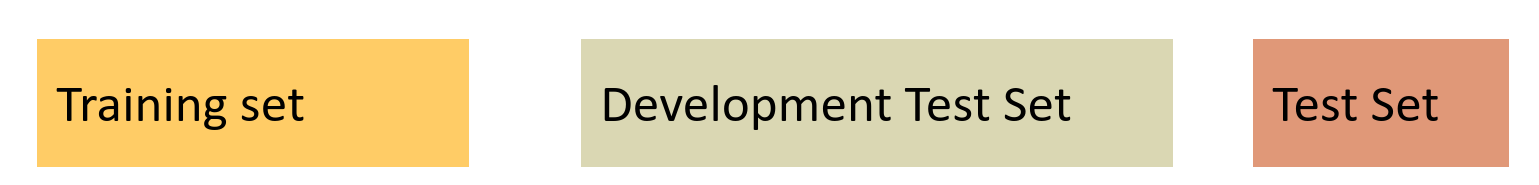
\includegraphics[scale = 0.23]{pics/devsets.png}
\end{figure}

\begin{itemize}
\item \textbf{Training set}: Used to train the model.
\item \textbf{Devset}: Used to tune the model and select the best hyperparameters.
\item \textbf{Testset}: Used to report the final performance of the model.
\end{itemize}


\item This approach ensures that the model is not tuned specifically to the test set, avoiding overfitting.
\item However, it creates a paradox: we want as much data as possible for training, but also for the devset.
\item How do we split the data?

\end{itemize}






\subsection{Cross-validation: Multiple Splits}

\begin{itemize}
\item Cross-validation allows us to use all our data for training and testing without having a fixed training set, devset, and test set.
\item We choose a number $k$ and partition our data into $k$ disjoint subsets called folds.
\item For each iteration, one fold is selected as the test set while the remaining $k-1$ folds are used to train the classifier.
\item We compute the error rate on the test set and repeat this process $k$ times.
\item Finally, we average the error rates from these $k$ runs to obtain an average error rate.
\item 10-fold cross-validation, for example, involves training 10 models on 90\% of the data and testing each model separately.
\item The resulting error rates are averaged to obtain the final performance estimate.
\item However, cross-validation requires the entire corpus to be blind, preventing examination of the data for feature suggestion or understanding system behavior.
\item To address this, a fixed training set and test set are created, and 10-fold cross-validation is performed within the training set.
\item The error rate is computed conventionally in the test set.
\end{itemize}




\begin{center}
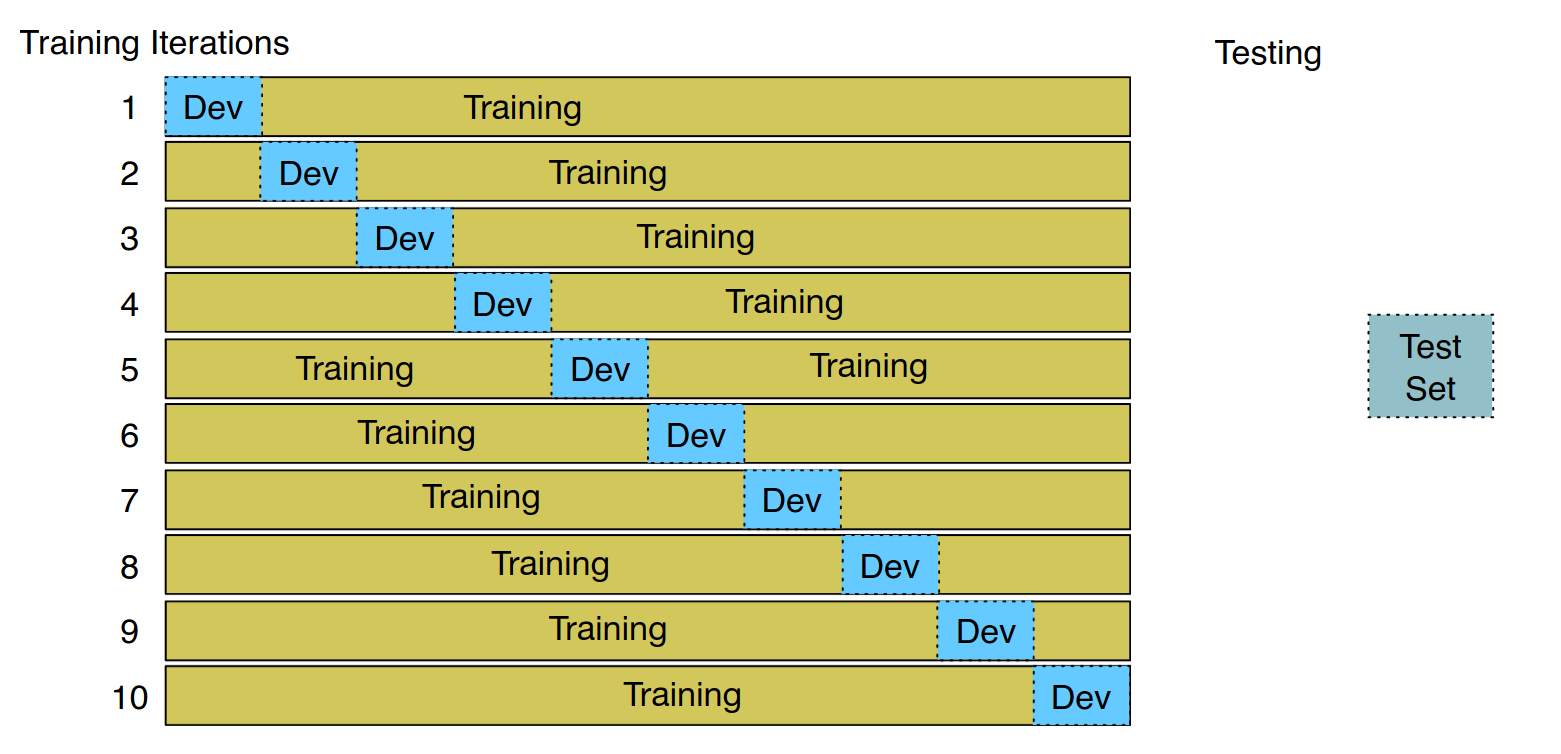
\includegraphics[scale=0.28]{pics/cv.png}
\end{center}




\subsection{Confusion Matrix for 3-class classification}


\begin{center}
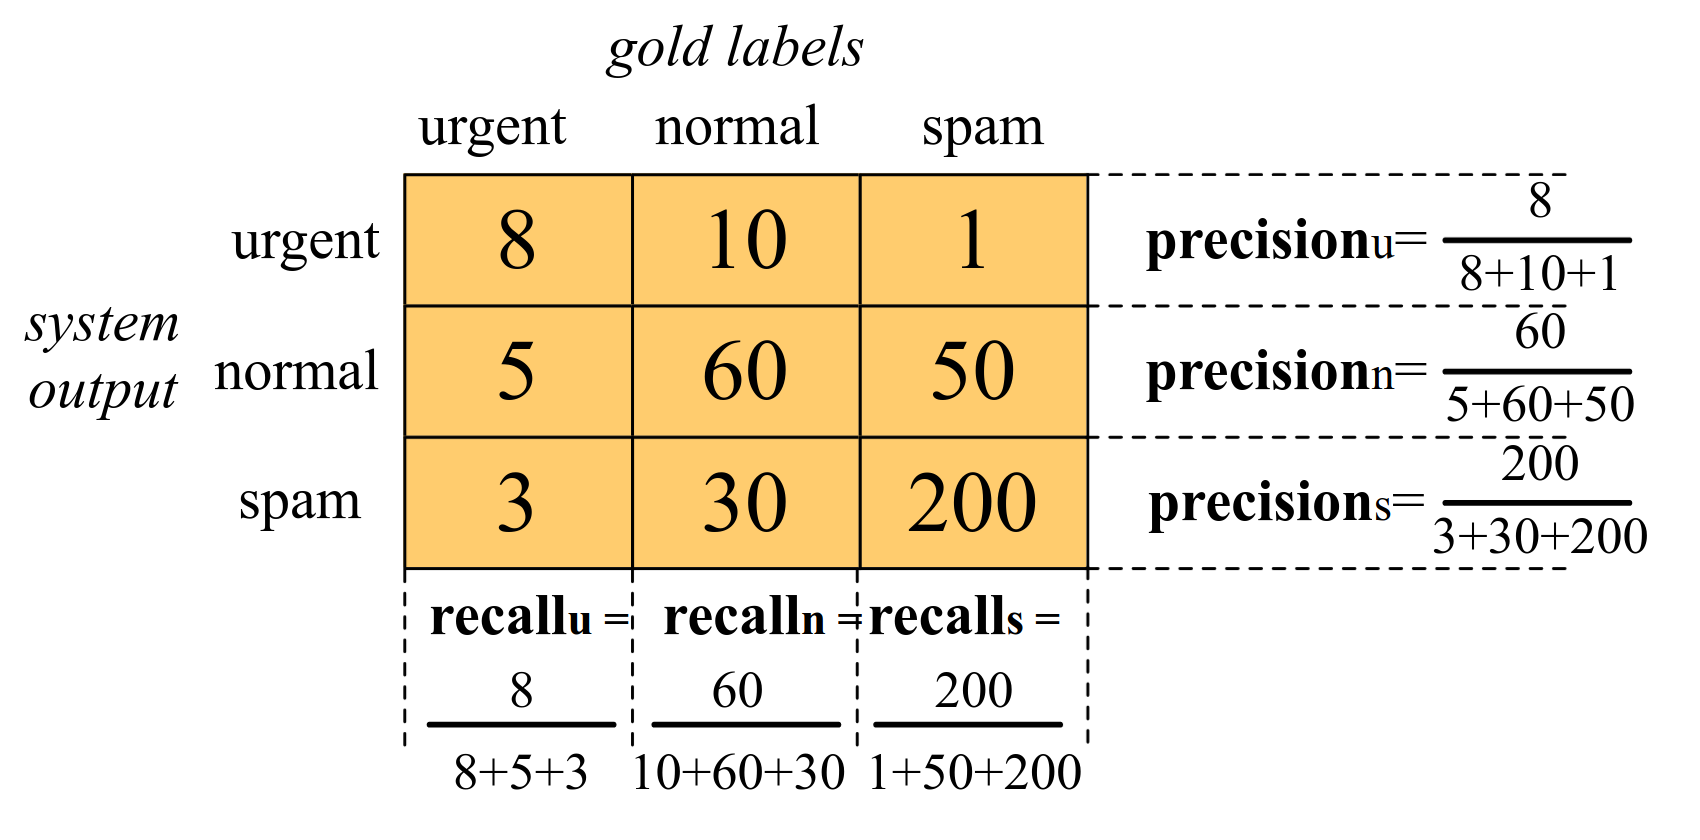
\includegraphics[scale=0.23]{pics/confmatrix.png}
\end{center}


How to combine binary metrics (Precision, Recall, $F_1$) from more than 2 classes to get one metric:
\begin{itemize}
 \item Macroaveraging:
 \begin{itemize}
    \item Compute the performance metrics (Precision, Recall, $F_1$) for each class individually.
    \item Average the metrics over all classes.
 \end{itemize}
 \item Microaveraging:
 \begin{itemize}
    \item Collect the decisions for all classes into one confusion matrix.
    \item Compute Precision and Recall from the confusion matrix.
 \end{itemize}
\end{itemize}



\begin{center}
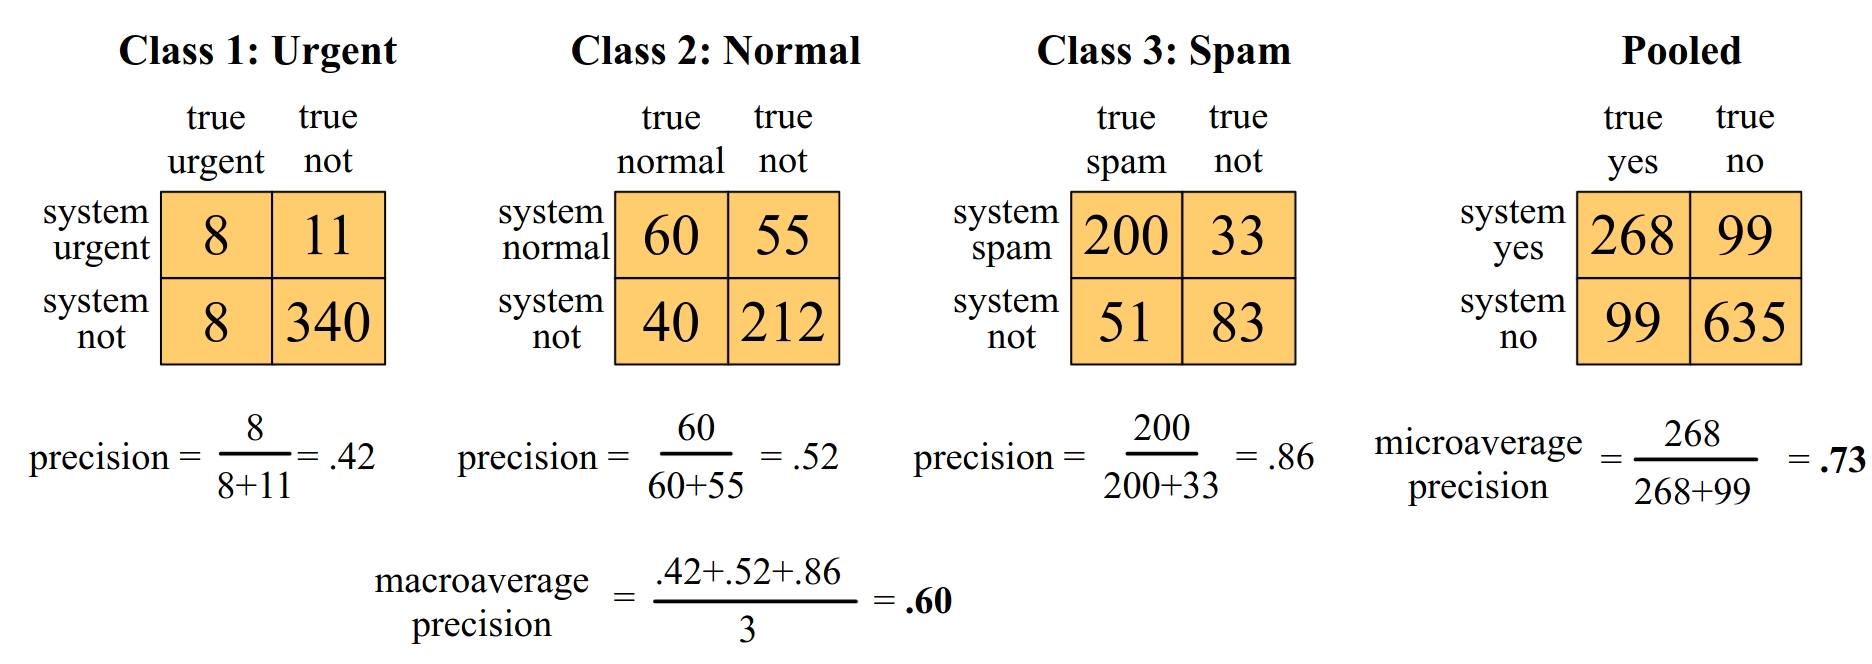
\includegraphics[scale=0.23]{pics/confmatrixmulti.png}
\end{center}
